\section{Control Module}

The control module is responsible for coordinating the activity of the
other parts of the image processor and transferring data into 
the image processor. A visual overview of the control module is given in
Figure \ref{fig:control-module}.

\begin{figure}[h!]
\centering
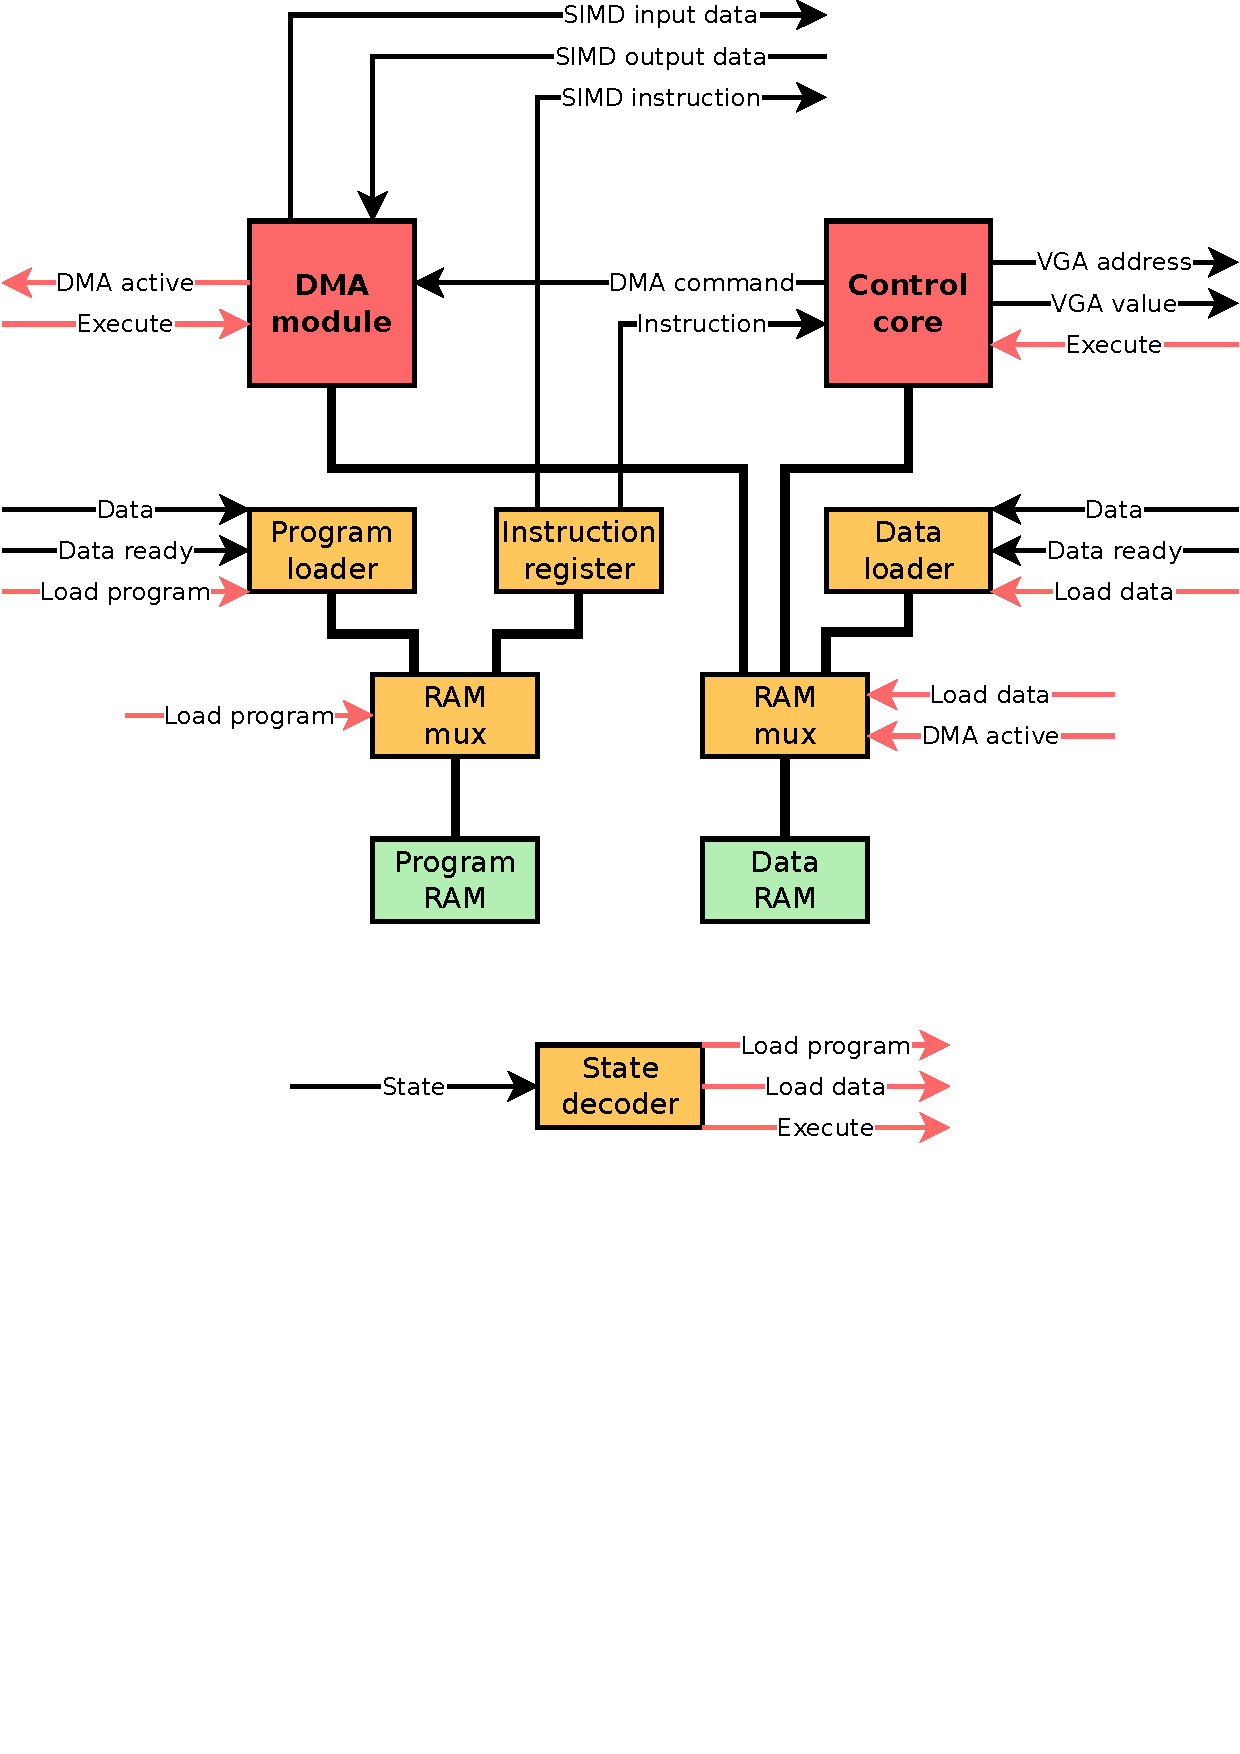
\includegraphics[width=\linewidth,clip,trim=0 10cm 0 0]
                {fig/fpga/control_module.pdf}
\caption[Control module]
        {An overview of the control module of the image processor.}
\label{fig:control-module}
\end{figure}


The control module decodes the state signal set by the SCU, and enables,
disables and resets components accordingly. It is responsible for performing
data transfers between the SCU, the program and data memories, and for
transferring data internally between the \ac{SIMD} node array, data \ac{RAM}
and the \ac{VGA} screen buffer. %\TODO{Isn't this the DMA's work?}

The control module contains the \ac{CPU} that is used for the non-\ac{SIMD}
instructions embedded in a program. This \ac{CPU}, henceforth referred to as the
\emph{control core}, is mainly concerned with loop control, initiating data
transfers between the \ac{SIMD} node array and the data RAM, and copying image
data to the \ac{VGA} controller.

\subsection{States}

The operation of the image processor is fully controlled by the \ac{SCU}. The
\ac{SCU} sets a state value that is used by the control module to select which
components of the image processor are active. This is indicated by the red
signals\CHECK{Må skrives ut i farge om vi skal ha dette med} in Figure
\ref{fig:control-module}.

The states recognized by the image processor are listed in Table
\ref{tab:states}.

\begin{table}[h]
  \centering
  \begin{tabular}{cl}\toprule
    \thx{State} & \thx{Description} \\ \midrule
    000 & Idle \\
    001 & Run program \\
    010 & Load data from SCU \\
    100 & Load program from SCU \\
    \bottomrule
  \end{tabular}
  \caption{Image processor states.}
  \label{tab:states}
\end{table}


\subsection{Control Core}

A schematic overview of the control core is given in Figure
\ref{fig:fpga-ctrl-core}. The control core consists of a register bank
of 21 bit registers, an \ac{ALU} and a connection to the data \ac{RAM}. The word
width of 21 bits was chosen to match the address width of the data \ac{RAM}.
This allows the control core to do pointer arithmetic referring to
arbitrary words in the data \ac{RAM}.

\begin{figure}[h]
  \centering
  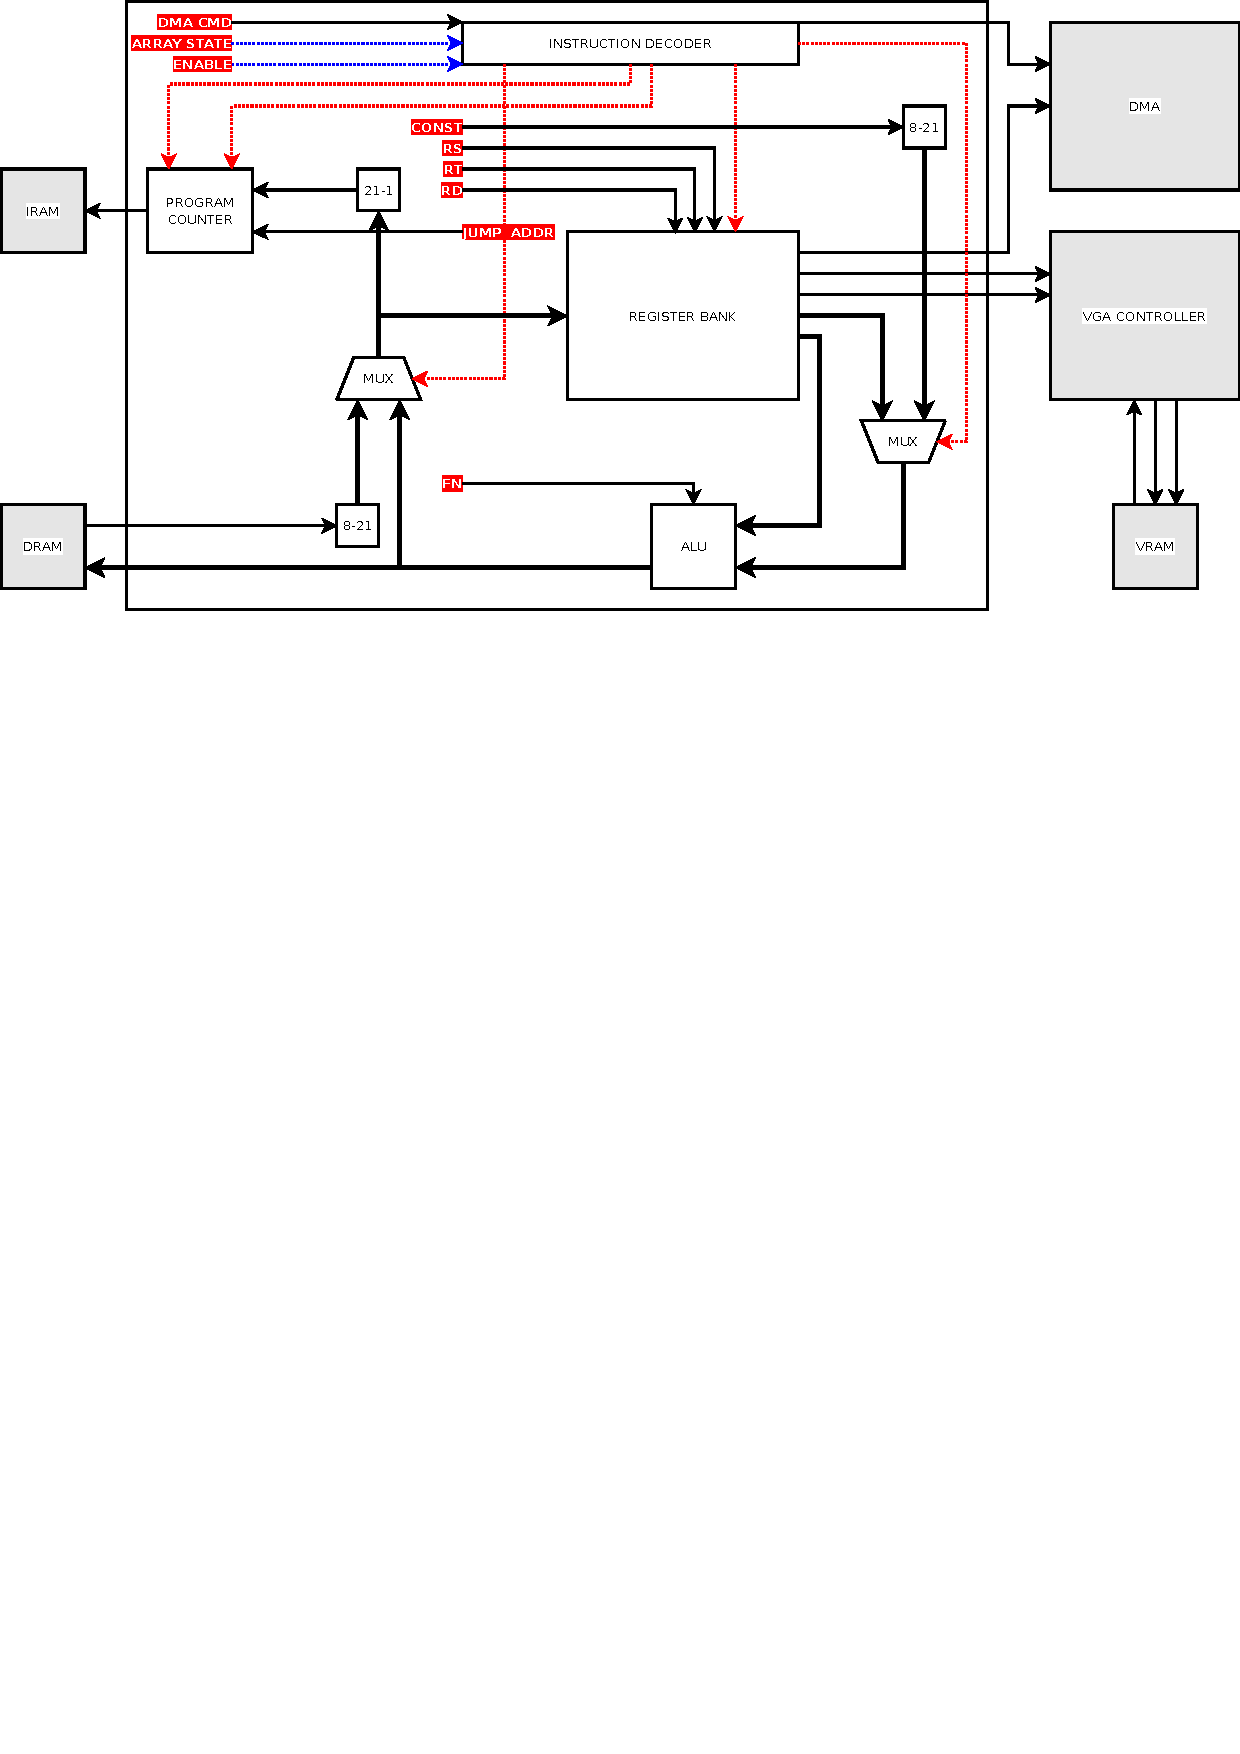
\includegraphics[width=\linewidth,clip,trim=0 18cm 0 0]
                  {fig/fpga/fpga_ctrl_core.pdf}
  \caption{Image processor control core.}
  \label{fig:fpga-ctrl-core}
\end{figure}

To send pixels to the \ac{VGA} controller, two of the registers are dedicated to
contain an address and a pixel value, respectively. The contents of these
registers are constantly sent to the \ac{VGA} controller. By incrementing and
loading \ac{RAM} values into these registers, using the control core's regular
instruction set, the control core program can upload images to the \ac{VGA}
screen buffer.

A third register is wired to the \ac{DMA} controller, to enable 21 bit wide
\ac{DMA} parameters to be set programmatically.

The control core runs instructions from the same instruction stream as the
\ac{SIMD} nodes, and thus the control core and the \ac{SIMD} array share a
common program counter. The leftmost bit in the instructions specifies whether
the instruction is a control core instruction or a \ac{SIMD} instruction.

\subsection{DMA Module}

Because of the common instruction stream between the \ac{SIMD} array and the
control core, the \ac{SIMD} array will be inactive whenever the control core is
busy. An important task that normally would be the control core's responsibility
is to load the \ac{SIMD} array with new data from \ac{RAM} and to store the
processed data back to \ac{RAM}. To maximize the utilization of the data
\ac{RAM} \ac{I/O} capacity and the processing power of the \ac{SIMD} array, a
\emph{Direct Memory Access module} was devised, allowing us to overlap
computation and communication.

The \ac{DMA} module performs loading of new \ac{SIMD} data planes and storing of
processed \ac{SIMD} data planes \emph{in parallel} with the normal execution of
program instructions. The S registers in the \ac{SIMD} nodes are reserved for
the \ac{DMA} module, and the module can send the contents of the S registers one
step to the right by setting a \emph{step S} signal.

With these accommodations of the \ac{SIMD} array, the \ac{DMA} module can load
new data values to the S registers at the left edge of the \ac{SIMD} array, send
the step signal to have these value propagate into the array and read the old,
processed data values from the S registers at the right edge of the array. The
\ac{SIMD} program executing simultaneously will operate on a different set of
registers and will not be obstructed by the \ac{DMA} data transfer.

During \ac{DMA} transfer, the data \ac{RAM} is reserved for the \ac{DMA} module
and is not available for the control core. To initiate a \ac{DMA} transfer, the
control core sets \emph{base addresses} for the reading of new data and for the
writing of old data, in addition to address increments to be used for moving
along the columns and rows of the current slice of the data. These parameters
allow flexibility in how the data slices are laid out in memory.
% to be loaded into and stored out of the \ac{SIMD} array, 
% ^ dragged out, as it is implicit.
